\documentclass[conference, 10pt]{IEEEtran}
\IEEEoverridecommandlockouts
% The preceding line is only needed to identify funding in the first footnote. If that is unneeded, please comment it out.
\usepackage{cite}
\usepackage{amsmath,amssymb,amsfonts}
\usepackage{algorithm,algorithmic}
\usepackage{graphicx}
\usepackage{textcomp}
\usepackage{xcolor}
\usepackage{url}
\usepackage[hidelinks]{hyperref}
\usepackage{hhline}
\usepackage{verbatim}
\usepackage{array}
\def\BibTeX{{\rm B\kern-.05em{\sc i\kern-.025em b}\kern-.08em
   T\kern-.1667em\lower.7ex\hbox{E}\kern-.125emX}}
   
\begin{document}

\newcommand{\Fix}[1]{\textbf{[[#1]]}}
\newcommand{\Code}[1]{\begin{small}\texttt{#1}\end{small}}

% This two commands changes spacing between equations
\setlength{\belowdisplayskip}{2pt} \setlength{\belowdisplayshortskip}{2pt}
\setlength{\abovedisplayskip}{3pt} \setlength{\abovedisplayshortskip}{3pt}
 
% This command reduces spacing below single column figure and tables
\setlength{\textfloatsep}{0.6\baselineskip plus 0.2\baselineskip minus 0.2\baselineskip}

% This command reduces spacing above foot notes
\setlength{\skip\footins}{3pt}

% IMPORTANT: 论文撰写中的一些约定
% 1. 对于论文内容的重要评论和TODO,使用\Fix命令,会在正文醒目标出
% 2. 对于论文内容的次要评论和提示,直接留下注释即可
% 3. 对于需要用等宽字体的场合,使用\Code命令

\title{A Multi-Metric Ranking Approach for Library Migration Recommendations}

\author{\IEEEauthorblockN{Hao He\IEEEauthorrefmark{1}\IEEEauthorrefmark{2},
Yulin Xu\IEEEauthorrefmark{1}, Yixiao Ma\IEEEauthorrefmark{1},
Yifei Xu\IEEEauthorrefmark{1}, Guangtai Liang\IEEEauthorrefmark{2},
and Minghui Zhou\IEEEauthorrefmark{1}\textsuperscript{\textsection}}

\IEEEauthorblockA{\IEEEauthorrefmark{1}Department of Computer Science and
Technology, Peking University, Beijing, China\\
\IEEEauthorrefmark{1}Key Laboratory of High Confidence
Software Technologies, Ministry of
Education, China\\
\IEEEauthorrefmark{2}Software Analysis Lab, Huawei Technologies Co., Ltd., China\\
Email: \{heh, kylinxyl, mayixiao, xuyifei, zhmh\}@pku.edu.cn\IEEEauthorrefmark{1},
liangguangtai@huawei.com\IEEEauthorrefmark{2}}}

\maketitle

\begingroup\renewcommand\thefootnote{\textsection}
\footnotetext{Minghui Zhou is the corresponding author.}
\endgroup

\begin{abstract}
%% background
The wide adoption of third-party libraries in software projects is beneficial but also risky. 
An already-adopted third-party library may be abandoned by its maintainers, may have license incompatibilities, or may no longer align with current project requirements. 
% Open-source third-party libraries are widely used to increase the efficiency of software development. However, developers need to update or migrate these libs in time due to several reasons, e.g., vulnerability remediation, license compliance, performance improvements.
Under such circumstances, developers need to migrate the library to \textit{another library} with similar functionalities, but the migration decisions are often opinion-based and sub-optimal with limited information at hand.
Therefore, several filtering-based approaches have been proposed to mine library migrations from existing software data to leverage ``the wisdom of crowd,'' but they suffer from either low precision or low recall with different thresholds, which limits their usefulness in supporting migration decisions.

%% our work
In this paper, we present a novel approach that utilizes multiple metrics to rank and therefore recommend library migrations.
Given a library to migrate, our approach first generates candidate target libraries from a large corpus of software repositories, and then ranks them by combining the following four metrics to capture different dimensions of evidence from development histories: Rule Support, Message Support, Distance Support, and API Support. % 改了回去,还是觉得开发历史更客观
We evaluate the performance of our approach with 773 migration rules (190 source libraries) that we borrow from previous work and recover from 21,358 Java GitHub projects. 
The experiments show that our metrics are effective to help identify real migration targets, %from other libraries, 
and our approach significantly outperforms existing works, with MRR of 0.8566, top-1 precision of 0.7947, top-10 NDCG of 0.7702, and top-20 recall of 0.8939.
To demonstrate the generality of our approach, we manually verify the recommendation results of 480 popular libraries not included in prior work, and we confirm 661 new migration rules from 231 of the 480 libraries with comparable performance. %%%zhmh: 单纯读这句话,get不到point
The source code, data, and supplementary materials are provided at: \url{https://github.com/hehao98/MigrationHelper}.
\end{abstract}

\begin{IEEEkeywords}
library migration, mining software repositories, library recommendation, multi-metric ranking
\end{IEEEkeywords}

\section{Introduction}

% 库很重要
Modern software systems rely heavily on third-party libraries for rich and ready-to-use features, reduction of development cost and productivity promotion~\cite{1994IEEESoftware-Lim-Effects, 2007ESEM-Mohagheghi-Quality}. 
In recent years, the rise of open-source software and the emergence of package hosting platforms, such as GitHub~\cite{GitHub}, Maven Central~\cite{Maven} and NPM~\cite{NPM}, has led to an exponential growth of open source libraries.
For example, the number of newly-published JARs in Maven Central is 86,191 in 2010, 364,268 in 2015, and over 1.2 million in 2019~\cite{Maven}. 
Nowadays, open-source libraries can satisfy a diverse spectrum of development requirements, and are widely adopted in both commercial and open-source software projects~\cite{2020ICSME-Wang-Empirical}.

\begin{figure}
  \centering
  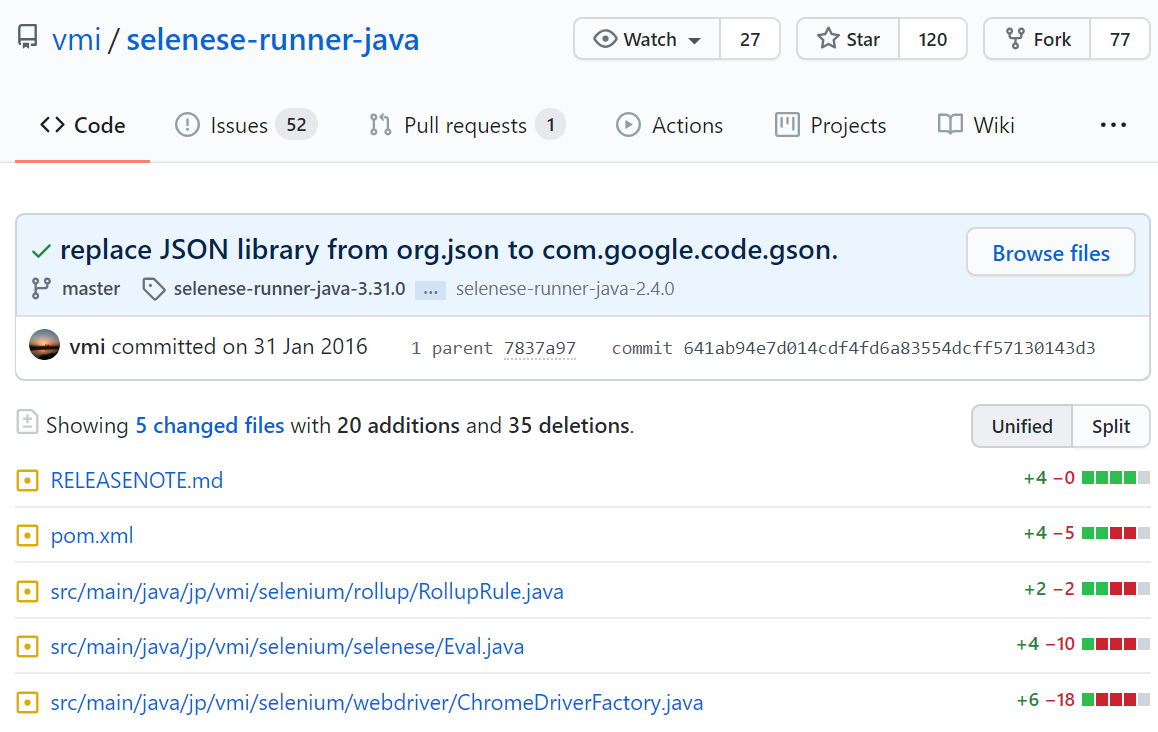
\includegraphics[width=0.4\textwidth]{fig/example.png}
  \caption{An example migration between JSON libraries}
  \label{fig:example}
\vspace{-2mm}
\end{figure}

% 为什么需要替换库
However, third-party libraries are known to cause problems during software evolution.
% third-party libraries are free to use, however managing these libs costs very much due to the following issues:  
First, third-party libraries may have sustainability failures~\cite{2017FSE-Coelho-Why, 2018FSE-Valiev-Ecosystem}. 
They may be abandoned by their maintainers due to lack of time and interest, difficulty in maintenance, or being superseded by competitors~\cite{2017FSE-Coelho-Why}. 
Second, third-party libraries may have license restrictions~\cite{2012IEEESoftware-German-Method, 2014ASE-Van-Tracing}. If a project uses a GPL-licensed library during early prototyping, it must be replaced before the project is released as proprietary software.
% Second, third-party libraries may have security vulnerabilities~\cite{2018MSR-Decan-On, 2019USENIXSec-Zimmermann-Small}, and in practice fixes are not always available at certain time or context. 
Finally, third-party libraries may fail to satisfy new requirements due to absence of features, performance issues, etc. 
Suppose a Java application at its infancy stage is using \Code{org.json:json}~\cite{orgjson} for its simplicity. 
When the application matures and scales, it often has to migrate to another JSON library for richer features or higher performance (see Figure~\ref{fig:example} for an example). 
To address any of these issues, software projects have to replace some already-used libraries (i.e., source libraries) with some other similar or functionality-equivalent libraries (i.e., target libraries). Such activities are  called as \textit{library migration} in the related literature~\cite{2012WCRE-Teyton-Mining, 2013WCRE-Teyton-Automatic, 2014JournalOfSysAndSoft-Teyton-Study, 2016MSR-Kabinna-Logging, 2019ICPC-Alrubaye-On, 2019ICSME-Alrubaye-MigrationMiner, 2019Arxiv-Alrubaye-How, 2020ASC-Alrubaye-Learning}.

% 替换库的难点,为什么要自动推荐
However, it is often not easy to find good target libraries and choose between a number of candidate libraries~\cite{2012WCRE-Teyton-Mining, 2016SANER-Chen-Mining, 2018PROMISE-Mora-An}.  
Community curated lists such as \Code{awesome-java}~\cite{awesome-java} and AlternativeTo~\cite{alternative-to} are often non-informative and contain low quality libraries, while blog posts and articles tend to be opinion based and outdated~\cite{2016SANER-Chen-Mining}. 
The easily accessible metrics such as popularity and release frequency have limited usefulness and they vary with domain~\cite{2018PROMISE-Mora-An}. 
In practice, industry projects often rely on domain experts for making migration decisions~\cite{2020FSE-Larios-Selecting}, while open source projects only migrate libraries when core developers reach a consensus in discussions~\cite{2016MSR-Kabinna-Logging}. In either case, the migration is not guaranteed to be appropriate, cost-effective or beneficial to the project.

%%%然后下面就是讨论这些automated recommendation appropoach工作
To address these challenges, researchers have proposed
several approaches to mine library migrations from existing software data~\cite{2012WCRE-Teyton-Mining, 2014JournalOfSysAndSoft-Teyton-Study, 2019ICSME-Alrubaye-MigrationMiner}. The underlying rationale is that historical migration practices provide valuable reference and guidance for developers when they make migration decisions, and the optimal decisions can be discovered from ``the wisdom of crowd'' if the analyzed software corpus is large enough and of high quality.
Their approaches first mine candidate migration rules from a large number of projects, and then filter the candidates based on frequency~\cite{2012WCRE-Teyton-Mining} or related code changes~\cite{2019ICSME-Alrubaye-MigrationMiner}. However, their approaches suffer from either low recall~\cite{2012WCRE-Teyton-Mining, 2019ICSME-Alrubaye-MigrationMiner}, or low precision~\cite{2012WCRE-Teyton-Mining, 2014JournalOfSysAndSoft-Teyton-Study} for two reasons.
First, a global filtering threshold is defined but not equally effective for all migration scenarios, thus hard to reach a performance balance. 
Second, valuable information sources are not considered in their filtering metrics.
The usefulness of existing approaches is also limited, because a low precision will result in high human inspection effort, while a low recall prevents developers from making optimal decisions because some migration opportunities may be missed.
% (See Section \ref{sec:related-work} for comparison with other related works)

To improve the effectiveness of these approaches~\cite{2012WCRE-Teyton-Mining, 2014JournalOfSysAndSoft-Teyton-Study, 2019ICSME-Alrubaye-MigrationMiner}, we propose a new approach for automated recommendation of library migration targets from existing software development histories.
%Therefore, we propose a new approach for automated recommendation of library migration targets that makes better use of the wisdom of crowd to achieve better results.
Instead of mining and filtering, we formulate this problem as a \textit{mining} and \textit{ranking} problem, because we observe that relative ranking positions are not only more important but also more robust to metric and parameter changes.
Given a source library, our approach first \textit{mines} target library candidates from the dependency change sequences (defined in Section~\ref{subsec:bg-terminoligies}) built from a large corpus of software development histories. 
After that, the candidates are \textit{ranked} based on a combination of four carefully designed metrics: Rule Support, Message Support, Distance Support and API Support.
The metrics are designed to capture different sources of evidence from data and pinpoint likely migration targets based on the evidences.
Finally, the top target libraries, their metrics, and the relevant migration instances are returned for human inspection.
Our approach is implemented as a web service, which can be used by project maintainers to seek migration suggestions or support their migration decisions. 

To implement our approach, we collect version control data of 21,358 Java GitHub repositories %from the World of Code database~\cite{2019MSR-Ma-WorldOfCode}, where we
and successfully extract 147,220 dependency change sequences from their dependency configuration files.
% \footnote{In a Maven managed project, a \texttt{pom.xml} file declares all libraries used in a project folder. We do not consider Gradle managed projects in the evaluation.}.
To support metric computation, we also collect Maven artifacts from Maven Central~\cite{Maven} using Libraries.io~\cite{LibrariesIO}, and extract API information for each collected Maven artifact. 
To evaluate the performance of our approach, we recover and extend migration rules in~\cite{2014JournalOfSysAndSoft-Teyton-Study} from the collected 21,358 repositories and get %an initial 
a ground truth of 773 migration rules (190 source libraries).
We use the 190 source libraries as query to our approach, which returns 243,152 candidate rules along with their metrics. The candidate rules include all ground truth migration rules mentioned above.
%During the evaluation, we first demonstrate the effectiveness of each metric by comparing metric distributions of ground truth migrations (extended from previous work~\cite{2014JournalOfSysAndSoft-Teyton-Study}) with distributions of other candidates.
Then, we estimate and compare survival functions for each metric, and compute Mean Reciprocal Rank (MRR)~\cite{Craswell2009MRR}, top-$k$ precision, top-$k$ recall and top-$k$ Normalized Discounted Cumulative Gain (NDCG)~\cite{2002-NDCG} for our approach along with existing approaches and a number of other baselines.
Finally, we experiment our approach on additional 480 popular libraries both to ensure our approach is generalizable and to confirm more real world migrations.
Our experimental evaluations show that the metrics are effective to help identify real migration targets from other libraries, the method that combines all four metrics can reach MRR of 0.8566, top-1 precision of 0.7947, top-10 NDCG of 0.7702 and top-20 recall of 0.8939 in the ground truth dataset, and we confirm 661 new migration rules with comparable performance.
% Our initial deployment in an industry setting obtains positive feedback.
Our approach has been deployed in a proprietary 3rd-party library management tool to recommend migration targets for libraries in the deny list.
%We also extend the migration dataset in Teyton et al.~\cite{2014JournalOfSysAndSoft-Teyton-Study} with both new migration rules and latest migration commits for existing rules, resulting in a total of 1,384 migration rules in 3,340 commits from 1,313 repositories. The new migration dataset can be used to facilitate further research in library migration.

We make the following contributions in this study:
\begin{enumerate}
    \item formulate the library migration recommendation problem as a \textit{mining} and \textit{ranking} problem, 
    \item propose a new multi-metric ranking approach via mining dependency change sequences, which significantly outperforms existing approaches,
    \item implement and conduct a systematic evaluation for our approach, showing that the approach is effective in suggesting migration targets for Java Maven projects,
    \item provide a latest ground truth dataset of 1,384 migration rules and 3,340 related commits discovered from 1,651 open source Java projects. The dataset can be used to facilitate further research in library migration.
\end{enumerate}

\section{Background}

We first provide a brief introduction to the context of our approach. 
% We first introduce the context of our approach.
%After that, we define common terminologies and a dependency model used throughout the remainder of this paper. Then, we provide our definition to the library migration recommendation problem. 
We then define common terminologies and a dependency model, and formulate the library migration recommendation problem. 
Finally, we discuss the existing approaches provided by Teyton et al.~\cite{2012WCRE-Teyton-Mining, 2014JournalOfSysAndSoft-Teyton-Study} and Alrubaye et al.~\cite{2019ICSME-Alrubaye-MigrationMiner}, before introducing our approach in the next section.

\subsection{Library Migration}

Migration is a common phenomenon in software maintenance and evolution, and may refer to different development activities that stem from various motivations. 
Common cases of migrations in software development include: migrating from a legacy platform to a modern platform~\cite{2007MODEL-Fleurey-Model, 2019SANER-Verhaeghe-GUIMigration}, one programming language to another programming language~\cite{2013FSE-Nguyen-Lexical, 2014ASE-Nguyen-Statistical, 2015ASE-Nguyen-DivideAndConquer, 2016ICSE-Nguyen-Mapping, 2016ICSM-Nguyen-Context, 2017SANER-Dorninger-Multi, 2019FSE-Bui-SAR}, one library version to another library version \cite{2012FSE-Cossette-Seeking, 2018EMSE-Kula-Do}, one API to another API \cite{2010ICSE-Nita-Using, 2010OOPSLA-Kapur-Refactoring, 2013WCRE-Teyton-Automatic, 2013ICSE-Gokhale-Inferring, 2014TOSEM-Santhiar-Mining, 2015ICSME-Hora-Apiwave, 2019ICPC-Alrubaye-On, 2019TSE-Chen-Mining}, or one library to another library \cite{2009SLE-Bartolomei-Study, 2010ICSM-Bartolomei-Swing, 2012WCRE-Teyton-Mining, 2014JournalOfSysAndSoft-Teyton-Study, 2016MSR-Kabinna-Logging, 2019ICSME-Alrubaye-MigrationMiner}. 
In this paper, we use the term \textbf{library migration} to refer to the process of replacing one library with another library of similar functionalities, as in \cite{2012WCRE-Teyton-Mining, 2013WCRE-Teyton-Automatic, 2014JournalOfSysAndSoft-Teyton-Study, 2016MSR-Kabinna-Logging, 2019ICPC-Alrubaye-On, 2019ICSME-Alrubaye-MigrationMiner, 2019Arxiv-Alrubaye-How, 2020ASC-Alrubaye-Learning}.

Two steps are typically needed for a library migration. The first step is to decide which library to migrate to and whether a migration is worthy. 
The second step is to conduct the real migration by modifying API calls in source code, changing configuration files, etc\footnote{See Section \ref{sec:related-work} for related work about the second step.}. 
For example, Kabinna et al.~\cite{2016MSR-Kabinna-Logging} study logging library migrations in Apache Software Foundation (ASF) projects. 
They discover that ASF projects conduct logging library migrations for flexibility, new features and better performance, but the code changes are hard and bug-prone, and 
some projects fail to migrate due to absence of submitted patches or lack of maintainers' consensus. 
% Alrubaye et al.~\cite{2019Arxiv-Alrubaye-How} found that library migrations are likely to improve several software quality metrics in Java projects, but it will take 2-42 days for a project to conduct a migration~\cite{2020ASC-Alrubaye-Learning}.
Given current situation, the main objective of our approach is to provide \textit{explainable} and \textit{evidence based} support to the first step of migration, such that developers can make the most appropriate migration decision for their project based on the recommendation results.
As introduced earlier, the existing approaches to achieve this goal suffer from low precision or low recall, and limited usefulness in practice.

\subsection{Terminologies and Dependency Model}
\label{subsec:bg-terminoligies}

% We largely reuse the terminologies and dependency model from previous work~\cite{2012WCRE-Teyton-Mining,2014JournalOfSysAndSoft-Teyton-Study, 2019ICSME-Alrubaye-MigrationMiner}. 
Let $\mathcal{P}$ be the set of projects and $\mathcal{L}$ be the set of libraries to be analyzed. 
A project $p\in\mathcal{P}$ has a set of revisions $Rev(p)=\{r_1,r_2,...,r_n\}$, where each revision has zero, one or more parent revisions. 
We define $r_i < r_j$ if $r_i$ happens before $r_j$ in $p$, and vice versa.
For each revision $r_i \in Rev(p)$, it depends on a set of libraries $L_i \subset \mathcal{L}$, which we call \textbf{dependencies} of $r_i$. 
By comparing with its parent revision(s) (e.g. $r_{i-1}$), we can extract the dependency changes of $r_i$ as\footnote{We will discuss how we deal with multi-parent revisions in Section \ref{sec:impl}.}
\begin{align}
L_i^+ &= L_i - L_{i-1} \\
L_i^- &= L_{i-1} - L_i 
\end{align}
where $ L_i^+$ is the set of added libraries and $ L_i^-$ is the set of removed libraries. By sorting all revisions in topological order and aggregating dependency changes, we can build a \textbf{dependency change sequence} $D_p$ for project $p$.
\begin{equation}
    D_p= L_1^+, L_1^-, L_2^+,  L_2^-, ...,  L_n^+,  L_n^- 
\end{equation}
We use the term \textbf{dep seq} as an abbreviation of \textbf{dependency change sequence} in the subsequent paper.

For library $a\in\mathcal{L}$ and library $b\in\mathcal{L}$, we consider $(a,b)$ as a \textbf{migration rule} if and only if $\exists p \in P,\ r_i, r_j \in Rev(p)$, $p$ has conducted a migration from $a$ to $b$ between $r_i$ and $r_j$, where $b \in  L_i^+$ and $a \in  L_j^-$. 
Note that a migration may either happen in one revision ($r_i = r_j$), or spans over multiple revisions ($r_i < r_j$). 
We refer to $a$ as \textbf{source library} and $b$ as \textbf{target library} in the subsequent paper.

\begin{figure}
  \centering
  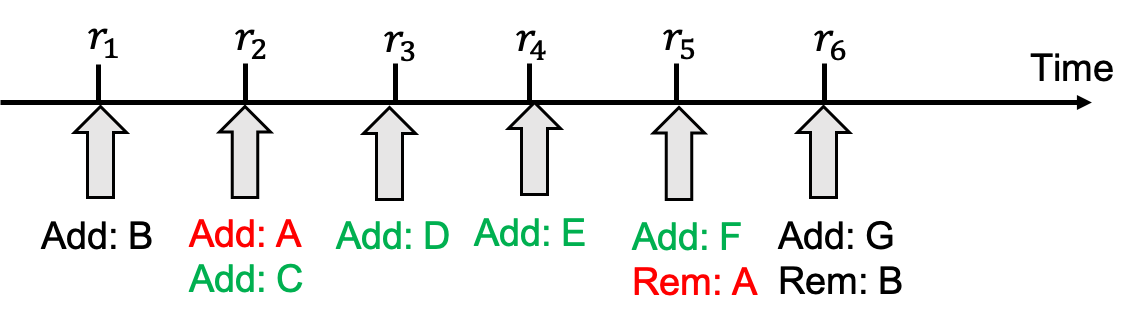
\includegraphics[width=0.4\textwidth]{fig/depseq.png}
  \caption{An example dependency change sequence}
  \label{fig:depseq}
\end{figure}

Figure~\ref{fig:depseq} shows an artificial example of a dependency change sequence where a project performs a migration from library $A$ to $F$ in revision $r_5$. 
In this case, $L_5^+=\{F\}$ and $L_5^-=\{A\}$, and $(A, F)$ is a migration rule by our definition.

\subsection{Problem Formulation}
%\subsection{Formulation of Library Migration Recommendation Problem}

We formulate the problem of library migration recommendation as follows.
Let $R$ be the set of all migration rules. 
Given projects $\mathcal{P}$, libraries $\mathcal{L}$, dep seqs $D_p$ for $p \in \mathcal{P}$, and a set of library queries (i.e. source libraries) $Q$, the objective of \textit{library migration recommendation} is to identify migration rules with both high coverage (for objectivity) and accurate results (for minimizing human inspection effort). 
For library $a \in Q$, an approach should seek to find \textbf{migration targets} $T=\{b|(a,b)\in R\}$. We view this problem as a two-step mining and ranking problem. In the mining step, an approach should generate a \textbf{candidate rule} set $R_c$ from all dep seqs. In the ranking step, for all $(a,b)\in R_c$, it should compute a confidence value $conf(a,b)$ and sort $R_c$ by this value. It should ensure that the target libraries in top ranked candidate rules are more likely to be real migration targets.

\begin{table*}[]
\caption{Comparison with most related work~\cite{2012WCRE-Teyton-Mining,2014JournalOfSysAndSoft-Teyton-Study,2019ICSME-Alrubaye-MigrationMiner}. See Section \ref{sec:evaluation} for more performance comparisons.}
\centering
\begin{tabular}{|l|m{45mm}|l|m{50mm}|}
\hline
 \textbf{Approach} & \textbf{Candidate Rules for $A$ in Figure \ref{fig:depseq}} & \textbf{Migration Rule Selection} & \textbf{Reported Performance}  \\ 
 \hhline{|=|=|=|=|}
 Teyton et al.~\cite{2012WCRE-Teyton-Mining} & $(A,F)$ & $conf_T(a,b) \ge 0.06$ & 0.679 precision, 80 migration rules \newline confirmed in 38,588 repositories\\ \hline
 Teyton et al.~\cite{2014JournalOfSysAndSoft-Teyton-Study} & $(A,C)$, $(A,D)$, $(A,E)$, $(A,F)$ & All candidate rules & 0.019 precision, 329 migration rules \newline confirmed in 15,168 repositories\\ \hline
 Alrubaye et al.~\cite{2019ICSME-Alrubaye-MigrationMiner} & $(A,F)$ & $RS(a,b) = 1 \land AC(a,b) > 0$ & 1.000 precision, 6 migration rules \newline confirmed in 16 repositories \\ \hline
 Our Approach &  $(A,C)$, $(A,D)$, $(A,E)$, $(A,F)$ & Rank by $conf(a,b)$ (Equation \ref{eq:conf}) & 0.795 top-1 precision, 1,384 migration rules \newline confirmed in 21,358 repositories\\
 \hline
\end{tabular}
\label{tab:related-work}
\vspace{-5mm}
\end{table*}

\subsection{Existing Approaches}
\label{subsec:bg-existing}

%Several existing filtering-based approaches can be fit into this problem definition. 
%While several existing approaches address migration recommendation problem, %\footnote{Note that the same two authors also have works at method level~\cite{2013WCRE-Teyton-Automatic, 2019ICPC-Alrubaye-On}, but we are specifically comparing their works at library level~\cite{2012WCRE-Teyton-Mining, 2014JournalOfSysAndSoft-Teyton-Study, 2019ICSME-Alrubaye-MigrationMiner}. For \cite{2019ICSME-Alrubaye-MigrationMiner}, we ignore its method level functionalities during comparison.}, %%%%zhmh: i don't feel this is needed because the cited papers are clear about that.
%they adopt the idea of mining and filtering. 
In this section, we introduce several existing approaches under our problem formulation. %%zhmh: please check this sentence.
Teyton et al.~\cite{2012WCRE-Teyton-Mining} define candidate rules as the Cartesian product of added and removed libraries in the same revision. More formally, for project $p$,
\begin{align}
  \label{eq:cand-teyton2012}
  R_{ci}^p &= \{(a,b)|(a,b)\in  L_i^- \times  L_i^+, r_i \in Rev(p)\} \\
  R_c &= \bigcup_{p\in\mathcal{P}}\bigcup_{r_i\in Rev(p)} R_{ci}^p
\end{align}
And they define confidence value as the number of revisions a rule occurs divides the maximum number of all rules with same source or same target as follows.
% Our approach combines this metric with three other metrics to recommend migration target. %%%important to hav
\begin{equation}
\label{eq:conf-teyton}
    conf_T(a,b)=\frac{|\{r_i|(a,b)\in R_{ci}^p\}|}{\max(|\{(a,x)\in R_c\}|, |\{(x,b)\in R_c\}|)}
\end{equation}
It captures most frequent rules and is partially reused in our first metric $RS$ (Section~\ref{subsec:rs}).
Their approach requires manual specification of a threshold $t$, and they consider a candidate rule $(a,b)$ as a migration rule if and only if $conf_T(a,b)\ge t$. 
In their evaluation, by setting $t=0.06$, they confirm 80 migration rules with a precision of 0.679 in 38,588 repositories.

In their subsequent work~\cite{2014JournalOfSysAndSoft-Teyton-Study}, they also consider migrations that spans over multiple revisions, using the following definition of candidate rules
\begin{equation}
\label{eq:cand-teyton}
R_c=\bigcup_{p\in\mathcal{P}}\{(a,b)|(a,b)\in L_j^- \times  L_i^+, r_i\le r_j\}
\end{equation}
By this definition, $(A,C)$, $(A,D)$, $(A,E)$ and $(A,F)$ in Figure~\ref{fig:depseq} will all be considered as candidate rules given $A$ as source library. 
In the hope of covering as many migration rules as possible, they manually verify 17,113 candidate rules generated from 15,168 repositories, in which they successfully confirm 329 migration rules.

Alrubaye et al.~\cite{2019ICSME-Alrubaye-MigrationMiner} propose a tool called MigrationMiner, which uses the same candidate rule definition as in \cite{2012WCRE-Teyton-Mining}, but filters candidate rules by their relative frequency and whether API replacements occur in code changes. 
Their filtering strategy can be effectively described in our framework as Rule Support $RS(a,b)=1$ and API Count $AC(a,b)>0$ (See Section~\ref{sec:approach} for their definitions). 
The tool is tested on 16 repositories where 6 migration rules can be confirmed with 100\% precision. 
Table~\ref{tab:related-work} provides a summary and comparison of existing approaches along with ours.

\section{Our Approach}
\label{sec:approach}

%In this section, we introduce our approach for recommending library migration targets at a high level. 
%As mentioned before, we tackle this problem using a mining step and a ranking step.
Our approach for recommending library migration involves two steps, a mining step and a ranking step.
We first describe how candidate rules are mined for each dep seq. 
Then we detail how we design the four ranking metrics.
Finally, we describe the confidence value, ranking strategy, and the pseudo code for our final algorithm.

\subsection{Mining Candidate Rules} 

Given a library $a$, the first step of our recommendation algorithm is to find a set of candidate rules $\{(a, x)\}$, in which $x$ may be a feasible migration target. 
We follow a similar process like in~\cite{2014JournalOfSysAndSoft-Teyton-Study} for mining candidate rules $R_c$ (Equation \ref{eq:cand-teyton}), due to its high coverage.
Since it is known to generate many false positives, we will specifically consider candidate rules mined from the same revision ($R_{ci}^p$ in Equation \ref{eq:cand-teyton2012}) during metric computation. We also collect all the relevant revision pairs for each candidate rule $(a,b)$, defined as
\begin{equation}
    Rev(a,b)=\{(r_i,r_j)|a\in L_j^- \land b\in L_i^+ \land r_i\le r_j\}
\end{equation}

\subsection{Four Metrics for Ranking} %%%zhmh: note that the current writing is not easy for audience to get the justification of the metrics. but let's leave it what it is, and improve this kind of writing next time

\subsubsection{Rule Support} 
\label{subsec:rs}

For each candidate rule $(a,b)$, we define Rule Count $RC(a,b)$ as the number of times $a$ is removed and $b$ is added in the same revision:
\begin{equation}
    RC(a,b)=|\{ r_i | (a,b)\in R_{ci}^p, \forall p \in \mathcal{P}, r_i \in Rev(p) \}|
\end{equation}
We define Rule Support $RS(a,b)$ as Rule Count divides the maximum value of Rule Count for all candidate rules with $a$ as source library:
\begin{equation}
    RS(a,b)=\frac{RC(a,b)}{\max_{(a,x)\in R_c}RC(a,x)}
\end{equation}
This metric is basically a reuse of $conf_T(a,b)$ in Equation \ref{eq:conf-teyton}, based on the intuition that the most frequent same-revision dependency changes are more likely to be library migrations. 
We omit the second denominator because it can only be computed with a full-scale mining ($Q=\mathcal{L}$), which is costly given the current number of libraries.

\subsubsection{Message Support} 
\label{sec:message-support}

Besides the ``implicit'' frequency-based hint characterized by Rule Support, we observe that the ``explicit knowledge'' provided by developer written messages accompanying revisions (e.g. commit messages or release notes) is extremely valuable.
Therefore, we design the following heuristic to determine whether a revision pair $(r_i, r_j)$ seems to be doing a migration from $a$ to $b$:
\begin{enumerate}
    \item First, we split the names of $a$ and $b$ into possibly informative parts, because developers often use shortened names to mention libraries in these messages.
    \item For $r_i = r_j$, we check whether its message is stating a migration from $a$ to $b$.
    \item For $r_i \ne r_j$, we check whether the message of $r_i$ is stating the introduction of library $b$ while mentioning $a$, and whether the message of $r_j$ is stating the removal of $a$ as a cleanup.
\end{enumerate}
The checks are implemented via keyword matching of library name parts along with different hint verbs for migrations, additions, removals, and cleanups. 
For example, we consider words like ``migrate'', ``replace'', ``switch'' as hinting a migration. 
We also iteratively refined the keyword matching strategies using ground truth commits discovered in Section \ref{sec:evaluation}.

Let $h(r_i, r_j)\mapsto \{0,1\}$ be the heuristic function described above, where $h(r_i,r_j)=1$ when the messages are considered as indicating a migration by our heuristic.
We define Message Count $MC(a,b)$ as the number of revision pairs $(r_i, r_j)$ whose messages are indicating a migration from $a$ to $b$, where $b$ is added in $r_i$ and $a$ in removed in $r_j$:
\begin{equation}
    MC(a,b)=|\{(r_i,r_j) | (r_i,r_j) \in Rev(a,b) \land h(r_i, r_j)\}|
\end{equation}
And we further define Message Support $MS(a,b)$ as
\begin{equation}
    MS(a,b)=\log_2(MC(a,b)+1)
\end{equation}

\subsubsection{Distance Support} 

The previous two metrics do not take into consideration multi-revision migrations without any meaningful messages, but such cases may still be common because not all developers write high quality messages.
Based on the observation that most real target libraries are introduced near the removal of source library, we design the Distance Support metric to penalize the candidates that often occur far away.
Let $dis(r_i, r_j)$ be the number of revisions between revision $r_i$ and $r_j$ ($0$ if $r_i=r_j$). We define Distance Support $DS(a,b)$ as the average of the inverse square distances of all revision pairs $(r_i, r_j) \in Rev(a,b)$:
\begin{equation}
    DS(a,b)=\frac{1}{|Rev(a,b)|} \sum_{ Rev(a,b)}\frac{1}{(dis(r_i,r_j)+1)^2}
\end{equation}

\subsubsection{API Support}

Another strong information source of a library migration is the real code modifications and API replacements performed between the two libraries. To capture this, we define API Count $AC(a,b)$ as the number of code hunks\footnote{A hunk is a group of added and removed lines extracted by the diff algorithm of a version control system.} in $Rev(a,b)$ where the APIs (i.e. references to public methods and fields) of $b$ are added and the APIs of $a$ are removed. Then, we define API Support as
\begin{equation}
    AS(a,b)=\max(0.1,\frac{AC(a,b)}{\max_{(a,x)\in R_c}AC(a,x)})
\end{equation}
The reason for setting a minimum threshold is to make $AS$ more robust in case no API change is detected for some migration rules. It happens either because the code changes are not performed synchronously with dependency configuration files, or because some libraries can work solely with configuration files.
For example, a manual analysis of 100 migration commits from ground truth (Section \ref{subsec:ground-truth}) reveals that 45 migration commits do not contain any relevant API changes, in which 26 commits only modify \Code{pom.xml} files, 12 commits modify configuration files, and others modify code in a way that the library APIs are not co-changed in one hunk.
% %(e.g. the migration only need to modify configuration files or only changes the inner implementation of a specification). 
%We find that the choice of threshold values will not significantly impact the final performance in our ranking framework. %%0.1 is a bit confusing, in that circumstance, 0.1 can save the day?

\subsection{Recommending Migration Targets}
\label{subsec:rec-targets}

Our recommendation algorithm combines the four metrics introduced above to generate a final confidence value for all candidate rules, using a simple multiplication as follows:
\begin{equation}
    conf(a, b) = RS(a,b) \cdot MS(a,b) \cdot DS(a,b) \cdot AS(a,b)
\label{eq:conf}
\end{equation}
For each library query $l\in Q$, the corresponding candidate rules are sorted by this confidence value from the largest to smallest.
If the confidence values of some candidate rules are the same, we further sort them using $RS$.
Finally, the recommendation results along with the relevant revision pairs, grouped by each library query, are returned for human inspection. 
Algorithm~\ref{algo:rec} provides a full description of our migration recommendation algorithm.
% where the aforementioned process is achieved through one iteration of all projects and their dep seqs (line 6-14), and one iteration of all candidate rules (line 15-24).
After initialization of the required data structure (line 1-5), we generate the candidate rules and accumulate necessary data for metric computation in one iteration of all projects and their dep seqs (line 6-14). 
After that, the metrics and confidence values are computed through another iteration of all candidate rules (line 15-24).
% Finally, all the candidate rules are grouped by their source libraries and sorted by the confidence value, and returned. 
% For each candidate rule $(a,b)$, the algorithm can also return $Rev(a,b)$ along with $h(r_i, r_j)$ for any $(r_i,r_j)\in Rev(a,b)$, if necessary.

Several important optimizations can be applied to Algorithm~\ref{algo:rec}. 
First, the initialization in line 2-4 can be done lazily to avoid excessive memory consumption. 
Second, for a project with length $n$ dep seq, the iteration in line 6 can be efficiently done in $O(n)$ by reversely traversing through the dep seq while maintaining a set of removed libraries and relevant revisions. 
Finally, we can precompute $AC(a,b)$ for all $(a,b)\in \mathcal{L}\times \mathcal{L}$ through one iteration of all project diffs, to avoid costly and often repetitive on-demand computation of $AC(a,b)$.

\begin{algorithm}[t]
 \caption{Recommending Library Migration Targets}
 \label{algo:rec}
 \begin{algorithmic}[1]
 \renewcommand{\algorithmicrequire}{\textbf{Input:}}
 \renewcommand{\algorithmicensure}{\textbf{Output:}}
 \REQUIRE Projects $\mathcal{P}$, libraries $\mathcal{L}$ and library queries $Q$.
 \ENSURE For $a\in Q$, $R_c$ sorted by $conf(a,b)$.
  \STATE Initialize: $Rev(a,b) \leftarrow \emptyset$
  \FOR {$(a,b)\in\mathcal{L}\times\mathcal{L}$}
    \STATE Initialize: $RC(a,b) \leftarrow MC(a,b) \leftarrow DS(a,b) \leftarrow 0$
    \STATE Initialize: $AS(a,b) \leftarrow 0.1$
  \ENDFOR
  \FOR {$p\in\mathcal{P},a\in Q, b\in R_c^p, (r_i,r_j)\in Rev(a,b)$}
    \STATE $Rev(a,b)\leftarrow Rev(a,b) \cup (r_i,r_j)$
    \IF {$r_i=r_j$} 
      \STATE $RC(a,b) \leftarrow RC(a,b)+1$
    \ENDIF
    \STATE $MC(a,b) \leftarrow MC(a,b) + h(r_i, r_j)$
    \STATE $DS(a,b) \leftarrow DS(a,b) + 1 / (dis(r_i,r_j) + 1)^2$
    \STATE $AC(a,b) \leftarrow AC(a,b) + \text{getAPICount}(r_i, r_j)$
  \ENDFOR
  \FOR {$(a,b)\in R_c=\bigcup_{p\in\mathcal{P}}R_c^p$}
    \STATE $RS(a,b) \leftarrow RC(a,b) / \max_{(a,x)\in R_c}RC(a,x)$
    \STATE $MS(a,b) \leftarrow \log_2(MC(a,b)+1)$
    \STATE $DS(a,b) \leftarrow DS(a,b)/|Rev(a,b)|$
    \STATE $AS'(a,b) \leftarrow AC(a,b)/\max_{(a,x)\in R_c}AC(a,x)$
    \IF {$AS'(a,b)>AS(a,b)$}
      \STATE $AS(a,b) \leftarrow AS'(a,b)$
    \ENDIF
    \STATE $conf(a,b)=RS(a,b) \cdot MS(a,b) \cdot DS(a,b) \cdot AS(a,b)$
  \ENDFOR
 \RETURN For $a\in Q$, $R_c$ sorted by $conf(a,b)$
 \end{algorithmic} 
\end{algorithm}

\begin{figure*}[tb]
  \centering
  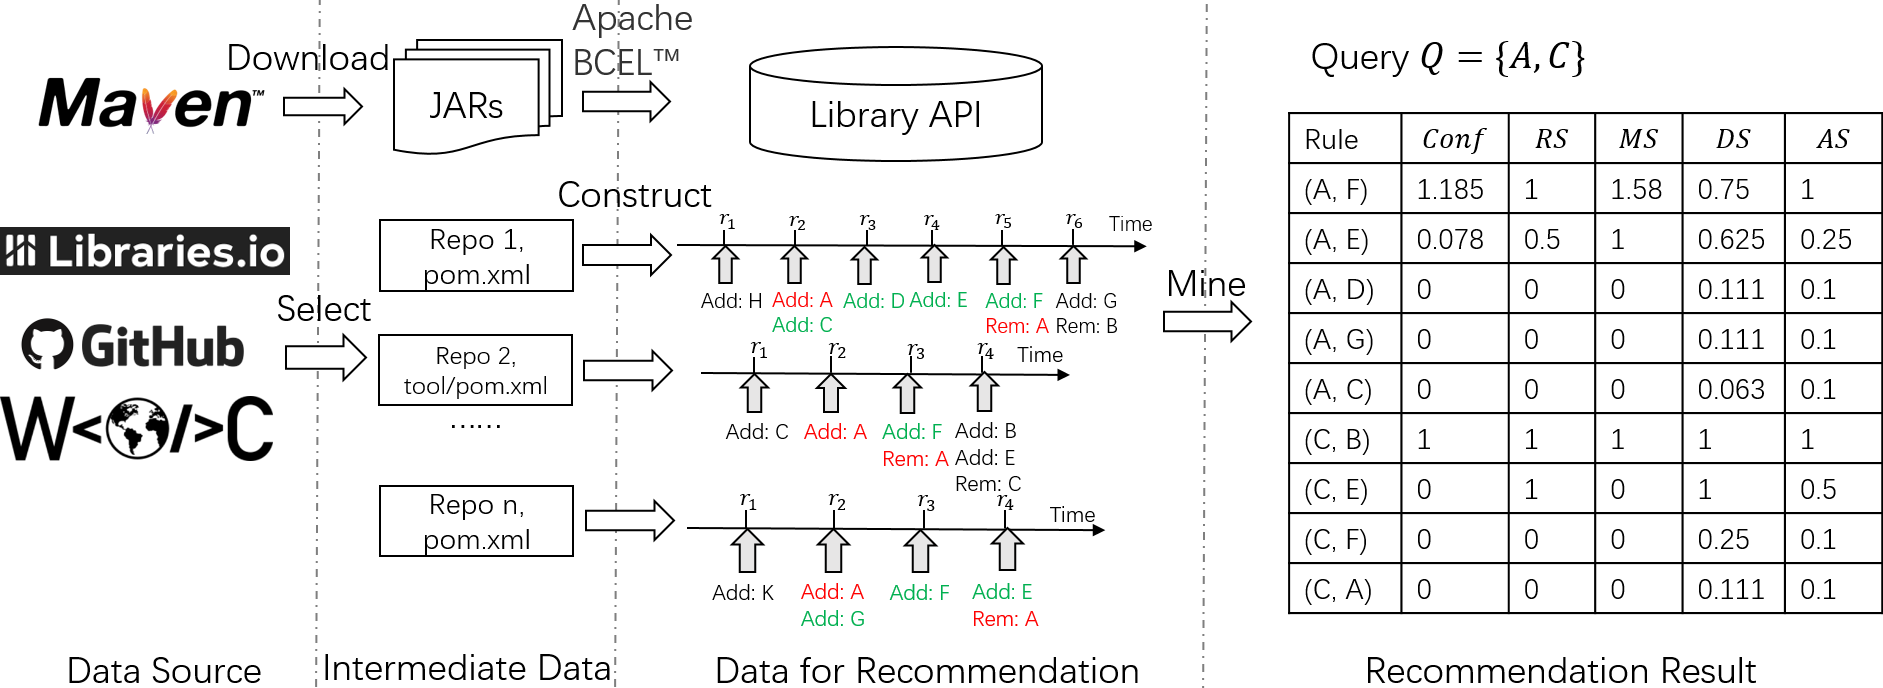
\includegraphics[width=0.8\textwidth]{fig/impl-overview2.png}
  \vspace{-1mm}
  \caption{Overview of the approach implementation, with some example data and results.}
  \label{fig:impl}
\vspace{-3mm}
\end{figure*}

% In Figure \ref{fig:impl}, there is an illustrative example for our algorithm, in which 9 candidate rules are generated for library $A$ and $C$ (i.e $Q=\{A, C\}$) based on 3 dep seqs. 

\section{Implementation}
\label{sec:impl}

In this section, we go through important implementation details for our approach, including design considerations, implementation environment, and the data collection process. Figure~\ref{fig:impl} provides an overview of our implementation.

\subsection{Design Considerations}
\label{subsec:design-consideration}

We choose to implement our approach for Java projects because of Java's popularity and industrial importance, and also because previous works~\cite{2012WCRE-Teyton-Mining, 2014JournalOfSysAndSoft-Teyton-Study, 2019ICSME-Alrubaye-MigrationMiner} are implemented for Java. 
We choose to mine dep seqs only for Maven~\cite{Maven-Tool} manged projects because it will make dependency extraction trivial by parsing the \Code{pom.xml} files. Each \Code{pom.xml} file has a dependency section where developers can declare used libraries by stating their library group IDs, artifact IDs and version numbers. 
During compilation, most declared libraries are downloaded from Maven Central~\cite{Maven}, which provides a central hosting service for most Java open source libraries indexed as ``artifacts.'' 
We consider artifacts with the same group ID and artifact ID as one library, and the version string as marking the different versions of a library.
We do not consider version number during recommendation.
Although multiple (group ID, artifact ID) may refer to the same library, we do not handle such aliases, because we observe that a renaming of group ID and artifact ID often accompanies important library changes, such as major version updates, intentional dependency shadowing, etc.
Therefore, we consider the migrations between such aliases as eligible migration rules.
However, we do not consider target libraries with the same group ID as source library, %%zhmh: ok, i'm confused here
because we observe that they are often siblings, sub-components or auxiliary libraries that are very unlikely to be a real migration target.

\subsection{Implementation Environment}

We implement our approach on a Red Hat Linux server with 2 Intel Xeon E5-2630 v2 CPUs, 400GB RAM and 20TB storage.
It has access to World of Code~\cite{2019MSR-Ma-WorldOfCode}, a database for storing open source version control data including almost all repositories from GitHub.
We use World of Code because it offers much higher performance when constructing dep seqs, compared with directly cloning from GitHub and analyzing with \Code{git}.
%The libraries and APIs are collected using Java, and the project dep seqs are constructed using Python. 
The data is constructed using a collection of Java programs and Python scripts, and stored in a local MongoDB~\cite{MongoDB} instance. 
The final recommendation service is implemented in Java using the Spring framework~\cite{Spring}.

\subsection{Data Collection}\label{ss:datacollection}

\subsubsection{Library Metadata and API Retrieval}

We use the Libraries.io dataset~\cite{LibrariesIO} (last updated in January 2020) to get a list of Maven artifacts and their metadata. 
After updating the latest version information from Maven Central in October 2020, we get a total of 184,817 distinct libraries for mining candidate rules, and 4,045,748 distinct library versions for API extraction.
Then, we download the corresponding JAR file from Maven Central for each version, if it has one. 
The total size of downloaded JAR files is $\sim$3TB, but they can be safely deleted after the APIs are extracted. 
For each JAR file, we use Apache Commons BCEL™ library~\cite{BCEL} to extract all public classes along with their fields and methods and store each class as a document in MongoDB.
Each document describes a unique and compact class signature object describing its fields, methods, inheritance relationships, etc.
They are indexed by SHA1 computed from all its properties. 
We also maintain mappings between library versions and classes. Finally, we get 25,272,024 distinct classes in total. 
The whole download and extraction process takes about 3 days to finish with 16 parallel threads on our server.

\subsubsection{Dep Seq Construction}

We use the GitHub repository list provided by the Libraries.io dataset, in which we select non-fork repositories with at least 10 stars and one \Code{pom.xml} file, resulting in 21,358 repositories.
We set the 10-stars threshold to ensure that the collected repositories are of sufficient quality.
The repository commits and blobs are then retrieved and analyzed from World of Code version R (last updated April 2020).
A repository may have multiple \Code{pom.xml} files in different paths for different sub-projects or sub-modules, so we consider each file as tracking the dependency of one project, and choose to construct one dep seq for each of the \Code{pom.xml} files.
For each \Code{pom.xml} file, we extract all commits where this file is modified, separately parse its old version and new version to see whether any library is added or removed. 
For merge commits, we only compare with one of its old version due to design and performance constraints.
For parallel branches, we sort changes by time and merge them into one dep seq. 
We then clean duplicate changes introduced by merge commits or parallel branches. After filtering out dep seqs with only one revision, we finally get 147,220 different dep seqs.

\subsubsection{API Count Precomputation}

As mentioned in Section \ref{subsec:rec-targets}, it is worthwhile to precompute an API Count table for each $(a,b)\in \mathcal{L} \times \mathcal{L}$, because on-demand computation during recommendation is not only time-consuming but also inefficient in that many Java file diffs will be analyzed multiple times for different candidate rules. 
Therefore, we iterate over all Java file diffs for each repository, while maintaining a set of current candidate rules, to see whether some of them should increment their API Count values.
The whole computation can be done in a highly parallel manner both for each repository and for code analysis of different Java file pairs.
In the end, we get 4,934,677 library pairs with non-zero $AC$ values.
The whole computation takes about two weeks to finish with 16 threads, but we believe it can be further optimized and only needs to be run once, because the table can be incrementally updated when new repository data come in. Table \ref{tab:db} provides an overview of the final recommendation database we use.

\begin{table}[]
\caption{Statistics of the recommendation database}
\centering
\begin{tabular}{|l|r|l|}
\hline
\textbf{Data Type} & \textbf{Count or Size} & \textbf{Time to Construct}  \\ \hhline{|=|=|=|}
GitHub repositories ($\mathcal{P}$) & 21,358 & Several minutes   \\ \hline
Commits with diffs                  & 29,439,998  & About 1 day  \\ \hline
Parsed \texttt{pom.xml}s            & 10,009,952  & About 1 day  \\ \hline
Dep seqs ($D_p$) & 147,220          & Several Hours \\ \hline
Libraries ($\mathcal{L}$)           & 185,817  & Several Minutes  \\ \hline
Library versions                    & 4,045,748  & Several Hours  \\ \hline
Java classes                        & 25,272,024  & About 3 days  \\ \hline
Non-zero API counts                 & 4,934,677 & About 2 weeks \\ \hline
Database size (compressed)          & $\sim$100GB & About 3 weeks \\ \hline
\end{tabular}
\label{tab:db}
\end{table}

\section{Evaluation}
\label{sec:evaluation}

In this section, we first introduce two research questions for evaluation.
Then, we describe how we build two ground truth datasets for different evaluation purposes. 
At last we show the evaluation methods and results for each research question.

\subsection{Research Questions}

Our main goal is to evaluate the effectiveness of Algorithm~\ref{algo:rec} in recommending library migration targets.
Since the algorithm mainly relies on a confidence value computed from four metrics (Equation \ref{eq:conf}), we first verify the effectiveness of each proposed metric, forming the first research question:
\begin{itemize}
    \item RQ1: How effective is $RS$, $MS$, $DS$, and $AS$ in identifying real migration targets? %from other libraries?
\end{itemize}

Then, to show that our approach has good overall performance, %1) outperforms existing approaches, and 2) generalizes well in different datasets, 
we 
% borrow existing ground truth migration rules and common metrics to evaluate ranking problems, 
ask the second research question:
\begin{itemize}
    \item RQ2: What is the performance of our approach, %in the ground truth datasets, 
    compared with baselines and existing approaches?
\end{itemize}

% Finally, to ensure our approach is generalizable and provide a latest dataset for further library migration research, we ask the third research question:
% Finally, to better ensure our approach is generalizable, we establish an additional dataset with 500 popular projects and ask the third research question:
%\begin{itemize}
    %\item RQ3: How many additional migration rules can we confirm in a new set of queries?
    % \item RQ3: What is the performance of our approach on another set of queries?
%\end{itemize}

\subsection{Ground Truth}
\label{subsec:ground-truth}

We use two ground truth datasets for different evaluation purposes. 
The first is borrowed from previous work~\cite{2014JournalOfSysAndSoft-Teyton-Study} and recovered in the 21,358 repositories we collect.
This set of ground truth has reasonably good coverage for the source libraries in it, so we can compute accurate performance metrics and compare different approaches.
The second is manually verified from the recommendation results of our algorithm on the 21,358 repositories, with 480 most popular libraries as queries. 
We use this dataset to verify that our approach can generalize well on a new dataset and confirm real word migrations with comparable performance.
% while we also use it to compare the performance of our approach with existing approaches.
In the subsequent section, we refer to the first ground truth set as GT2014 and the second as GT2020.

\subsubsection{GT2014}
We choose to recover a new ground truth of migration rules based on the ground truth in~\cite{2014JournalOfSysAndSoft-Teyton-Study}, as the current situation may have significantly changed since its publication.
The ground truth in \cite{2014JournalOfSysAndSoft-Teyton-Study} consists of 329 ``abbreviated'' library name pairs which may correspond to multiple group IDs and artifact IDs. 
They solve the aforementioned library aliasing issue (Section \ref{subsec:design-consideration}) through manual abbreviation, but we consider it too costly to repeat this on the 180k libraries we collected. 
As the Maven artifact pairs before abbreviation is not provided in~\cite{2014JournalOfSysAndSoft-Teyton-Study}, we choose to map the rules back to group IDs and artifact IDs. 
To cover as much migration rules as possible, we consider all pairs in Cartesian product as possible rules for multiple mappings.
We also conduct reverse and transitive expansion of the rules until saturation (i.e. $(a,b)\in R \Rightarrow (b,a) \in R$, $(a,b)\in R \land (b,c)\in R \Rightarrow (a,c)\in R$), based on the intuition that libraries within one functionality category can be replaced with any  other library in the same category. We get 3,878 ``possible'' migration rules after extension.

Recall in Section~\ref{subsec:bg-terminoligies} that we define a migration rule as a rule that we can confirm at least one migration in one project, so the rules collected before may still contain many false positives by this definition. 
Therefore, we %use all source libraries in the rules as queries to our approach, 
collect all relevant commits for these rules, filter them by commit messages, and manually label the rules using the following criteria:
% to see whether we can find at least one commit pair performing the corresponding migration
% We use the following criteria to determine whether $(a,b)$ is a migration rule:
\begin{enumerate}
    \item If library $a$ and library $b$ provide obviously different functionalities, we label $(a,b)$ as false.
    \item For other rules, we manually check the ``most possible'' commits by applying the message matching algorithm in Section \ref{sec:message-support}. If there exist some messages stating a migration from $a$ to $b$, we label $(a,b)$ as true.
    \item Otherwise, we check the commit diffs for easily understood small commits, and only label $(a,b)$ as true when we can find at least one understandable commit performing a migration from $a$ to $b$.
\end{enumerate}
The labelling process is done by three of the authors with at least one year of Java development experiences.
They are asked to search any unfamiliar libraries on Google, read through relevant websites, and consult Java veterans in our social network, until they become familiar with the libraries.
To mitigate threats brought by manual labelling, we adopt a conservative labelling strategy and ensure all rules with true labels are double checked by the author with 3 years of Java experiences and 1 year of industry experiences.
We also manually check the top-20 recommendation results and add any new migration rules using the same labelling process.
% It is worth noting that the ground truth is constructed and continuously updated when we iteratively refine our approach, so we believe it has a reasonably good coverage for the source libraries in it.
Finally, we get a ground truth of 773 migration rules with 190 different source libraries, distributed in 2,214 commit pairs from 1,228 repositories. This set of migration rules are mainly used for performance evaluations and comparison with other approaches, and denoted as $R_t$ in the remainder of this section.

In RQ1 and RQ2, we use the aforementioned 190 source libraries in $R_t$ as the query to our approach ($|Q|=190$), which returns 243,152 candidate rules\footnote{The large number comes from Equation \ref{eq:cand-teyton} which considers all possible migrations that spans over multiple revisions.} ($|R_c|=243,152)$) along with the metrics, commits and confidence values. Note that the number of candidate rules is significantly larger than the size of ground truth rules ($|R_t|=773$), which makes an effective ranking absolutely necessary. The recommendation only takes several minutes to finish with precomputed API Count data.

\subsubsection{GT2020}

We select the most popular 500 libraries based on the number of repositories they have been added. After filtering out existing source libraries in $R_t$, we get 480 libraries.
We use them as query to our approach and collect their recommendation output, resulting in 383,218 candidate rules. 
To ensure that the migration rules we confirm are valuable for a broad audience and keep a reasonable amount of human inspection effort, we only inspect candidate rules that:
\begin{enumerate}
    \item occur in top-20 recommendation result,
    \item have been added in more than 10 repositories,
    \item have non-zero confidence values.
\end{enumerate}
After the filtering, we need to label 4,418 candidate rules in 12,565 \Code{pom.xml} file changes, 2,353 commit pairs and 1,313 repositories. 
We repeat the labelling process as described before, and we successfully confirm 661 migration rules in 1,233 commits and 785 repositories, for 231 (48.125\%) of the 480 libraries. 
In RQ2, we also use GT2020 to verify and compare the performance of our approach with existing approaches for the 231 libraries, despite its incompleteness.


By merging GT2014 and GT2020, we get 1,384 migration rules from 14,334 \Code{pom.xml} changes, 3,340 commit pairs and 1,651 repositories (7.73\% of the 21,358 repositories). 
If we consider top 20\% largest repositories in terms of commit numbers, 1,092 out of 4,271 repositories (25.57\%) have undergone at least one library migration.
Both percentages are higher than the reported percentage in \cite{2014JournalOfSysAndSoft-Teyton-Study} (5.57\% and 9.95\%), indicating that library migrations have become more prevalent in Java open source projects since 2014. The dataset is available on our project website (see Abstract).

\subsection{RQ1: How effective is RS, MS, DS, and AS in identifying real migration targets from other libraries?}

\begin{figure*}[tb]
  \centering
  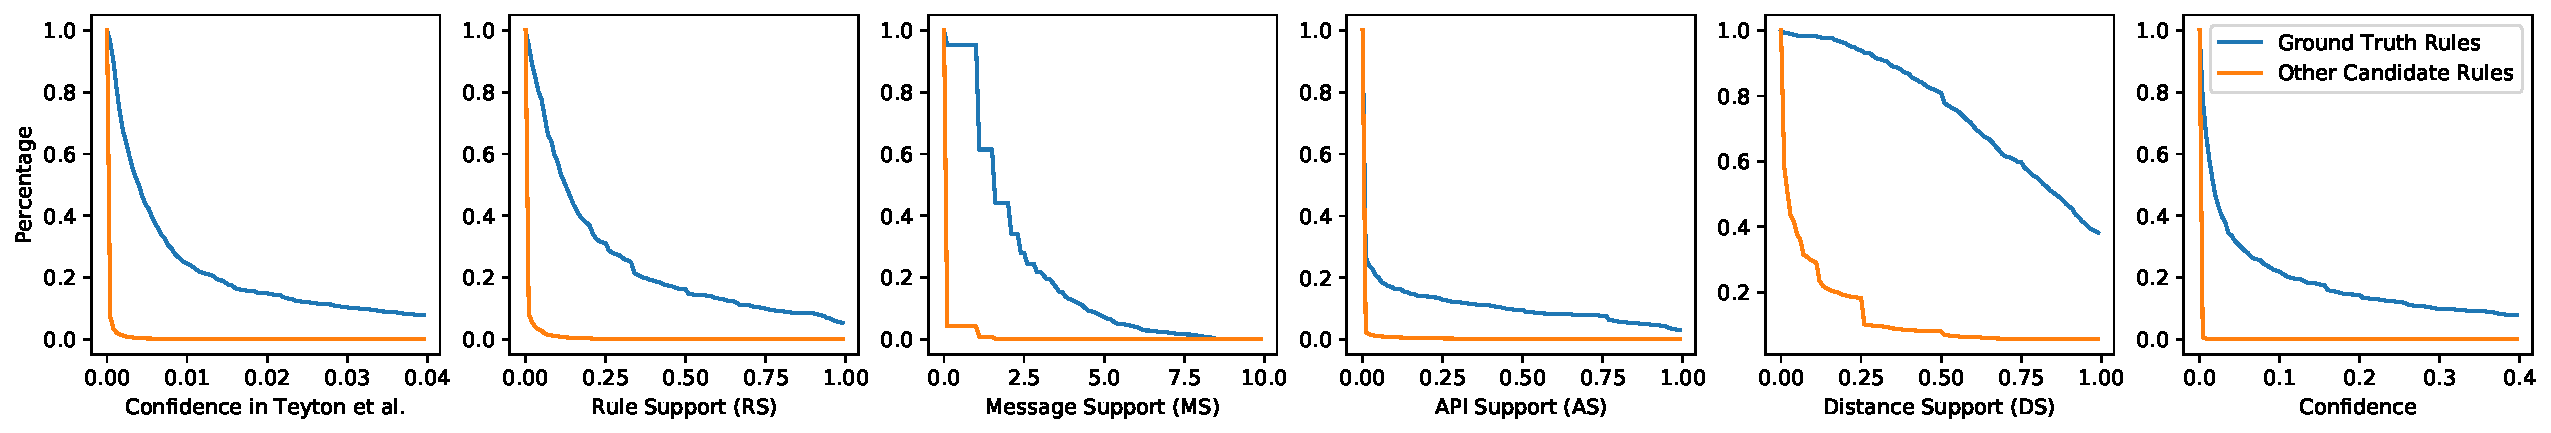
\includegraphics[width=0.95\textwidth]{fig/dist.pdf}
  \caption{The survival functions of ground truth rules and other rules. Note that the $0.1$ minimum threshold is not applied for $AS$ here.}
  \label{fig:dist}
\vspace{-5mm}
\end{figure*}

To answer RQ1, we plot survival functions for the confidence value of the approach in \cite{2012WCRE-Teyton-Mining},
the four proposed metrics, and the final confidence value of our approach, respectively. For metric $M$, its survival function is defined as $y=P(M\ge x)$, where $P()$ is the probability function.
We estimate the probabilities using GT2014, for both ground truth rules $R_t$ and other candidate rules $R_c-R_t$,
in Figure~\ref{fig:dist}. 
We can observe in Figure~\ref{fig:dist} that ground truth rules generally have significantly higher probability of survival for all metrics, indicating the effectiveness of each metric.
We can also observe that any filtering threshold $x$ will result in either significant ground truth losses or undesirable survival of many other candidate rules due to their much larger quantity.
Therefore, despite the effectiveness of each metric, we conclude that any filtering based method is inherently ineffective and we should leverage relative ranking positions instead of absolute metric values for selecting migration rules from the large number of candidates.
% The difference in steepness for ground truth rules and other rules can be clearly observed in each plot, but some are better in term of steepness (notably, $conf$ being the steepest among all plots). We can also observe the necessity of a minimum threshold for $AS$, as many ground truth rules have zero API Count values.

\subsection{RQ2: What is the performance of our approach compared with  baselines and existing approaches?}\label{ss:rq2}

\begin{table}[]
\caption{Performance comparison of different approaches in GT2014}
\centering
\begin{tabular}{|l|r|r|r|r|}
\hline
\textbf{Approach} & \textbf{MRR} & \textbf{Precision@1} & \textbf{NDCG@10} & \textbf{Recall@20}  \\ 
\hhline{|=|=|=|=|=|}
Teyton et al.            & 0.7133 & 0.6368 & 0.6056 & 0.7257 \\ \hline
Teyton et al.'           & 0.7335 & 0.6757 & 0.6909 & 0.6391 \\ \hline
Teyton et al.''          & 0.8858 & 0.8737 & 0.8909 & 0.1759 \\ \hline
Alrubaye et al.          & 0.9412 & 0.9412 & 0.9412 & 0.0540 \\ \hline
RS Only                  & 0.7208 & 0.6474 & 0.6073 & 0.7270 \\ \hline
MS Only                  & 0.7619 & 0.6737 & 0.6619 & 0.7736 \\ \hline
RS $\cdot$ MS            & 0.8275 & 0.7579 & 0.7436 & 0.8616 \\ \hline
RS $\cdot$ MS $\cdot$ DS & 0.8401 & 0.7737 & 0.7589 & 0.8680 \\ \hline
RS $\cdot$ MS $\cdot$ AS & 0.8379 & 0.7737 & 0.7479 & 0.8745 \\ \hline
Our Approach             & 0.8566 & 0.7947 & 0.7702 & 0.8939 \\ \hline
\end{tabular}
\label{tab:perf-comp}
\end{table}

For performance evaluation, we use the following quality metrics common for evaluating ranking problems: Mean Reciprocal Rank (MRR)~\cite{Craswell2009MRR}, top-$k$ precision, top-$k$ recall, and top-$k$ Normalized Discounted Cumulative Gain (NDCG)~\cite{2002-NDCG}. These metrics have also been used to evaluate other recommendation problems in software engineering~\cite{2013WCRE-Thung-Automated, 2014FSE-Ye-Learning, 2017JSS-Niu-API, 2017InfoSciAndTech-Ouni-Search}. 

Mean Reciprocal Rank (MRR) is defined as the mean of the multiplicative inverse of the rank of the first ground truth rule for all queries:
\begin{equation}
    MRR=\frac{1}{|Q|}\sum_{q \in Q}\frac{1}{\min_{(q,x)\in R_t} rank(q,x)}
\end{equation}
It ranges between $[0,1]$, and a higher value means that the user can see the first ground truth more quickly for each query.

Let $R_k$ be the top-$k$ ranked candidate rules for all queries, we define top-$k$ precision and top-$k$ recall as:
\begin{align}
    %Precision@k &= \frac{|R_k \cap R_t|}{|R_k|}\\
    %Recall@k &= \frac{|R_k \cap R_t|}{|R_t|}
    Precision@k &= |R_k \cap R_t| \mathbin{/} |R_k|\\
    Recall@k &= |R_k \cap R_t| \mathbin{/} |R_t|
\end{align}

Normalized Discounted Cumulative Gain (NDCG) measures to what extent the ranking result deviates from the ideal result. 
For each library $l \in Q$ and its top-$k$ returned rules $R_{lk}$, let $r(i)=1$ if the rank $i$ is in ground truth and 0 otherwise. 
By defining Discounted Cumulative Gain (DCG) as $DCG_l@k = \sum_{i=1}^k \frac{r(i)}{\log_2(i+1)}$ and Ideal Discounted Cumulative Gain (IDCG) as $IDCG_l@k = \sum_{i=1}^{|R_{lk}\cap R_t|} \frac{1}{\log_2(i+1)}$, we further define NDCG@k as
\begin{equation}
    NDCG@k=\frac{1}{|Q|}\sum_{l\in Q}\frac{DCG_l@k}{IDCG_l@k}
\end{equation}
which ranges in $[0,1]$ where $1$ means a perfect match with ideal top-$k$ ranking result and $0$ means the worst.

We first compare performance of our approach with the following alternatives using GT2014:
\begin{itemize}
    \item \textbf{Teyton et al.}~\cite{2012WCRE-Teyton-Mining}: Use $conf_T$ (Equation \ref{eq:conf-teyton}) for ranking.
    \item \textbf{Teyton et al.'}~\cite{2012WCRE-Teyton-Mining}: Keep rules $conf_T \ge 0.002$ and rank.
    \item \textbf{Teyton et al.''}~\cite{2012WCRE-Teyton-Mining}: Keep rules $conf_T \ge 0.015$ and rank.
    \item \textbf{Alrubaye et al.}~\cite{2019ICSME-Alrubaye-MigrationMiner}: Filter out $RS < 0.6$ or $AC = 0$.
    \item \textbf{RS Only}: Use only $RS$ for ranking.
    \item \textbf{MS Only}: Use only $MS$ for ranking.
    \item \textbf{RS $\cdot$ MS}: Use $RS \cdot MS$ for ranking.
    \item \textbf{RS $\cdot$ MS $\cdot$ DS}: Use $RS \cdot MS \cdot DS$ for ranking.
    \item \textbf{RS $\cdot$ MS $\cdot$ AS}: Use $RS \cdot MS \cdot AS$ for ranking.
\end{itemize}

% Some metric combinations are omitted because we find $DS$ and $AS$ only work well in combination with $RS$ and $MS$.
We choose three thresholds for Teyton et al.~\cite{2012WCRE-Teyton-Mining} to demonstrate its performance under different conditions, and tune parameters for Alrubaye et al.~\cite{2019ICSME-Alrubaye-MigrationMiner} to align with its reported performance.
We only show MRR, top-1 precision, top-10 NDCG and top-20 recall due to space constraints, where MRR and top-1 precision measures accuracy, top-10 NDCG measures idealness, and top-20 recall measures completeness\footnote{More results (including F-measures) are available on our project website.}.

The performance comparison results are shown in Table \ref{tab:perf-comp}. 
Our approach can outperform all alternatives in term of top-20 recall, while keeping high top-1 precision, MRR and top-10 NDCG. 
Although aggressive filtering approaches like Teyton et al.'' and Alrubaye et al. have higher precision, NDCG, and MRR\footnote{Note that precision, NDCG and MRR basically measures the same thing if only one or very few items are returned for each query.}, their recall is significantly lower than other approaches because of the filtering. 
The comparison with other metric combinations also shows that all four metrics are necessary to achieve the best performance. 
% The performance of Teyton et al.~\cite{2012WCRE-Teyton-Mining} is slightly lower than their reported result (Table \ref{tab:related-work}), and a possible reason is that they test their approach for releases while we test their approach for commits.
% However, because of the significant performance gap between their approach and ours, we believe such difference is negligible.
% Therefore, we conclude in Table \ref{tab:perf-comp} that our approach outperforms all existing approach and baselines in terms of MRR, top-10 NDCG and top-20 recall.
% There is only one exception that Alrubaye et al.~\cite{2019ICSME-Alrubaye-MigrationMiner} achieves higher top-1 precision using its aggressive filtering strategy (Section \ref{subsec:bg-existing}), but this strategy significantly impacts the recall and NDCG of its result.
Therefore, we conclude that our approach achieves the best overall performance and is the most suitable one for migration recommendation, compared with the evaluated alternatives.

To demonstrate the generality of our approach, we further compute the quality metrics using GT2020 for the 231 queries.
Since GT2020 is incomplete, we also show performance of Teyton et al.' for comparison.
Note that precision and MRR will be lower than their real values, and top-20 recall is 1 because we only check until top-20 results. 
However, we can still observe that our approach outperforms Teyton et al.' with a similar margin as in Table~\ref{tab:perf-comp}.
For example, the MRR of our approach is 13.1\% higher than Teyton et al.' in Table~\ref{tab:perf-comp2} and 16.8\% higher in Table~\ref{tab:perf-comp}.
% If we only consider candidate rules after filtering, our approach achieves comparable performance on all metrics in this new dataset (Note that it is trivial for users to apply similar custom filtering rules when using our service). 
% Even if we compute metrics for all rules (where some ground truth may be missed), we can still achieve reasonably good MRR and comparable top-10 NDCG values. 
Therefore, we conclude that our approach generalizes well in an unknown dataset.

%\subsection{RQ3: How many additional migration rules can we confirm in a new set of queries?}
% \subsection{RQ3: What is the performance of our approach on another set of queries?} 
%\label{ss:rq3}

\begin{table}[]
\caption{Performance of our approach in GT2020}
\centering
\begin{tabular}{|l|r|r|r|r|}
\hline
\textbf{Approach} & \textbf{MRR} & \textbf{Precision@1} & \textbf{NDCG@10} & \textbf{Recall@20}  \\ 
\hhline{|=|=|=|=|=|}
Teyton et al.'  & 0.6985 & 0.6035 & 0.6653 & 0.8020 \\ \hline
Our Approach    & 0.7902 & 0.6870 & 0.7770 & 1.0000 \\ \hline
\end{tabular}
\label{tab:perf-comp2}
\end{table}

\section{Recommendation Example}

\begin{table*}[]
\caption{Recommendation results of \texttt{c3p0:c3p0}. Migration commits are omitted here due to space constraints}
\centering
\begin{tabular}{|l|l|l|r|r|r|r|r|}
% \vspace{-0.3cm}
\hline
 \textbf{Rank} & \textbf{Is Correct} & \textbf{Library} & \textbf{Confidence} & $RS$ & $MS$ & $DS$ & $AS$  \\
 \hhline{|=|=|=|=|=|=|=|=|}
 $1$  & True  & com.mchange:c3p0                                          & 0.4083 & 0.9880 & 4.1700 & 0.9910 & 1.0000 \\ \hline
 $2$  & True  & com.zaxxer:HikariCP                                       & 0.0124 & 0.0238 & 1.0000 & 0.5222 & 0.1000 \\ \hline
 $3$  & False & org.jboss.jbossts.jta:narayana-jta                        & 0.0071 & 0.0357 & 2.0000 & 1.0000 & 0.1000 \\ \hline
 $4$  & False & org.springframework.boot:spring-boot-starter-test         & 0.0050 & 0.0595 & 1.0000 & 0.8518 & 0.1000 \\ \hline
 $5$  & True  & com.alibaba:druid                                         & 0.0039 & 0.0476 & 1.0000 & 0.8222 & 0.1000 \\ \hline
 $6$  & False & org.jboss.spec.javax.servlet:jboss-servlet-api\_3.0\_spec & 0.0038 & 0.0238 & 1.5849 & 1.0000 & 0.1000 \\ \hline
 $7$  & True  & org.hibernate:hibernate-c3p0                              & 0.0037 & 0.0357 & 1.5849 & 0.5430 & 0.1000 \\ \hline
 $8$  & False & org.hibernate:hibernate-core                              & 0.0030 & 0.0476 & 1.5849 & 0.3870 & 0.1000 \\ \hline
 $9$  & False & org.springframework.boot:spring-boot-starter-web          & 0.0029 & 0.0357 & 1.0000 & 0.7539 & 0.1000 \\ \hline
 $10$ & True  & com.alibaba:druid-spring-boot-starter                     & 0.0026 & 0.0238 & 1.0000 & 1.0000 & 0.1000 \\ \hline
 $11$-$14$ & False & All false positives, omitted due to space constraints  & - & - & - & - & - \\ \hline
 % $11$ & False & org.modeshape:modeshape-web-explorer                      & 0.0024 & 0.0238 & 1.0000 & 1.0000 & 0.1000 \\ \hline
 % $12$ & False & org.springframework.boot:spring-boot-devtools             & 0.0024 & 0.0238 & 1.0000 & 1.0000 & 0.1000 \\ \hline
 % $13$ & False & org.springframework.boot:spring-boot-starter-thymeleaf    & 0.0024 & 0.0238 & 1.0000 & 1.0000 & 0.1000 \\ \hline
 % $14$ & False & org.springframework.boot:spring-boot-starter-aop          & 0.0024 & 0.0238 & 1.0000 & 1.0000 & 0.1000 \\ \hline
 $15$ & True  & commons-dbcp:commons-dbcp                                 & 0.0012 & 0.0238 & 1.0000 & 0.3199 & 0.1667 \\ \hline
\end{tabular}
\label{tab:c3p0}
\vspace{-3.5mm}
\end{table*}

Table~\ref{tab:c3p0} presents one recommendation example from our results: \Code{c3p0:c3p0}. 
It is a database connection pooling library which has been renamed to \Code{com.mchange:c3p0} since version \Code{0.9.2} in 2007. 
Many other competitors for database pooling also emerged from 2007, under different licenses or for specific scenarios.
We choose \Code{c3p0:c3p0} as an example not only because of the diversity of migration targets returned, but also because it well demonstrates common failures and peculiarities of our approach. 
We can see from Table~\ref{tab:c3p0} that the top-1 recommended target is \Code{com.mchange:c3p0}, with much higher confidence than the rest.
The second result is Hikari CP, a database pooling library since 2013, which boasts its light-weight and much higher performance compared with other libraries. 
The 5th and 10th result is Alibaba Druid, a connection pool designed specifically for monitoring purposes. 
The 7th result is \Code{c3p0} for integrated use with Hibernate. 
The 15th result is Apache Commons DBCP, a pooling library under the ASF license. 
The rest of the results are omitted in the Table because they are all false positives.
Given the prevalence of migrations from \Code{c3p0:c3p0}, a developer should also consider abandoning it for his/her project, and choose one of the above libraries instead after evaluating the migration costs, benefits, licenses and other factors through investigation of the migration commits and other available information.

% Other candidates are ranked above some migration targets in Table \ref{tab:c3p0}, either because they are added together with the migration target in some migration commits, or because their commit messages are falsely identified as stating a migration.

\section{Limitations}
\label{sec:limitations}

\subsection{Failure Case Analysis}

\textbf{Cold Start}. 
The most obvious failure case in our approach is that, it can only recommend migration targets that have been frequently migrated in the project corpus. 
% Therefore, given a library $l$, even if $l'$ is a worthy migration target, our approach will not recommend $l'$ if few project in the project corpus has conducted a migration from $l$ to $l'$. 
However, this limitation can be mitigated by using a large project corpus, because the more worthy a migration is, the more common it will be in such a corpus. 
As shown in~\cite{2016MSR-Kabinna-Logging}, 33 of 223 ASF projects have undergone at least one logging migration, mostly from ad-hoc logging libraries (e.g. \Code{log4j}) to log abstraction libraries (e.g. \
\Code{slf4j}) and log unification libraries (e.g. \Code{logback}), and our approach performs well in these popular migrations. 
Developers can also conclude that a library is not a worthy migration target if it is absent in our result, even if it provides similar functionalities.
% Developers can also use other tools (e.g.~\cite{2016ASE-SimilarTech}) or Google search to come up with some alternatives, and use our tool to make the final decision.

\textbf{Data Sparsity}. 
Other failure cases are generally caused by the sparsity of many real migrations in our data. 
If only one or several relevant commits can be identified for a query, other added libraries in these commits tend to occur as false positives together with the true migration target (e.g. \Code{hibernate-core} in Table~\ref{tab:c3p0}).
$MS$ and $AS$ can handle such cases, but they sometimes fail either because developers do not write informative commit messages, or because code changes are not needed for the migration or are completed before/after the \Code{pom.xml} changes. 

\textbf{Miscellaneous}.
Our approach will fail if a library has no substitute at all, and it cannot issue any warnings in such cases.
Our method of matching commit messages sometimes falsely identify a migration, and can be improved by more sophisticated NLP techniques.
Our approach also frequently returns Bills of Materials, libraries that warp other libraries, or ``full solution'' frameworks like Spring in our results.
Even if they are not considered as migration targets during the labelling process, they may still be useful for developers.

\subsection{Threat to Validity}

\subsubsection{Construct Validity}

The metrics are mainly designed to achieve high performance in the formulated problem, and may not be a good indicator on the appropriateness or optimality of a given migration for a specific project.
Further research is needed to understand factors that drive library migrations, in order to design a better recommendation approach.
Even in term of performance, we cannot guarantee that the metrics we design and the parameters we choose are optimal.
To avoid over-fitting on a single dataset, we choose the simplest possible form for each metric, and evaluate our approach on an additional dataset.
For evaluation, it is generally impossible to compute accurate recall for all possible migration targets in the wild~\cite{2012WCRE-Teyton-Mining, 2014JournalOfSysAndSoft-Teyton-Study}. 
Even if we limit the evaluation on a set of ground truth libraries, we cannot guarantee completeness of the identified migration targets.
To mitigate this threat, we aggressively extend the largest set of migration rules from existing work~\cite{2014JournalOfSysAndSoft-Teyton-Study} and validate all extended rules, to present a ``best effort'' estimation of recall for GT2014 in RQ2.

\subsubsection{External Validity} 

Our approach may not generalize to a different dataset (e.g. industry projects) and to other programming languages and library ecosystems.
We mitigate this threat by collecting a large number of open source Java projects and libraries, and testing on many library queries. Also, our approach in Section~\ref{sec:approach} does not make any language specific assumptions and can be easily re-implemented for other programming languages. Others can also refer to Section~\ref{sec:impl} as an example of how to make implementation choices for a specific language or library ecosystem.

\section{Related Work}
\label{sec:related-work}

In this section, we go through related works not discussed before, and we summarize the relationship, differences or improvements of our work compared with theirs.

%Bartolomei et al.~\cite{2009SLE-Bartolomei-Study, 2010ICSM-Bartolomei-Swing} studied the feasibility, peculiarities, and design patterns of using API wrappers to migrate between two XML libraries~\cite{2009SLE-Bartolomei-Study} and two Java GUI libraries~\cite{2010ICSM-Bartolomei-Swing}. 
%They summarized peculiarities of designing wrapper libraries and proposed a set of design patterns for wrapper libraries.
%However, it is generally costly to implement a wrapper and nearly impossible to implement wrappers for all possible migrations.

To recommend libraries to developers, Thung et al.~\cite{2013WCRE-Thung-Automated} propose to recommend libraries based on the libraries a project is already using, through association rule mining and collaborative filtering.
More approaches are proposed for this problem later, such as multi-objective optimization~\cite{2017InfoSciAndTech-Ouni-Search},  hierarchical clustering~\cite{2018JSS-Saied-Improving}, advanced collaborative filtering~\cite{2020JSS-Nguyen-CrossRec}, matrix factorization~\cite{2020TSE-He-Diversified}, etc. 
%Ouni et al use  for recommendation of libraries.
However, their main objective is to recommend missed reuse opportunities based on the libraries a project is using and the properties of the project, not to recommend migration opportunities of a library already in use. 
Chen et al.~\cite{2016SANER-Chen-Mining} mine semantically similar libraries by training word embedding on Stack Overflow tags. Given a library, their method can return a list of possibly similar libraries, but it provides no evidence on the feasibility and prevalence of migrations between this library and the returned libraries.
% Based on the ideas of recommending migrations from existing migrations in the wild~\cite{2012WCRE-Teyton-Mining, 2014JournalOfSysAndSoft-Teyton-Study}, we establish our approach but focus on designing more effective metrics so that we can accurately recommend candidate libraries to migrate to.

Mora et al.~\cite{2018PROMISE-Mora-An} study the role of common metrics in developer selection of libraries. Alrubaye et al.~\cite{2019Arxiv-Alrubaye-How} analyze several code quality metrics before and after library migration. They all use existing metrics for empirical analysis, while we specifically design new metrics for accurate mining and recommendation of migrations from existing software data.

A number of studies have proposed methods for mining API mappings of two similar libraries~\cite{2011FSE-Zheng-Cross, 2013ICSE-Gokhale-Inferring, 2013WCRE-Teyton-Automatic, 2019ICPC-Alrubaye-On, 2019TSE-Chen-Mining, 2020ASC-Alrubaye-Learning} or directly editing code to use the new API~\cite{2019ICPC-Xu-Meditor,2020ASE-Collie-M3}. 
Zheng et al.~\cite{2011FSE-Zheng-Cross} mine alternative APIs from developer shared knowledge in forums or blog posts. 
Gokhale et al.~\cite{2013ICSE-Gokhale-Inferring} build mappings by harvesting the execution traces of similar APIs. 
Teyton et al.~\cite{2013WCRE-Teyton-Automatic} find API mappings by analyzing their co-occurring frequencies in existing migrations. 
Alrubaye et al. improve their method using information retrieval techniques~\cite{2019ICPC-Alrubaye-On} and machine learning models~\cite{2020ASC-Alrubaye-Learning}.
Chen et al.~\cite{2019TSE-Chen-Mining} propose an unsupervised deep learning based approach that embeds both API usage patterns and API descriptions.
Xu et al.~\cite{2019ICPC-Xu-Meditor} propose an approach to infer and apply migration edit patterns from existing projects.
Collie et al.~\cite{2020ASE-Collie-M3} propose to model and synthesize library API behavior without prior knowledge, which can be used for identifying migration mappings and applying migration changes.
The output of our approach can serve as input for any of the approaches above, because they all require manual specification of library pairs. Our new migration dataset may also be helpful in facilitating further research into this area.

Other recent works also aim to aid dependency management, but from a different perspective, such as characterizing library usage~\cite{2020ICSME-Wang-Empirical}, versioning ~\cite{2019TSE-Decan-Semantic, 2019MSR-Dietrich-DependencyVersioning, 2019MSR-Valero-DiversityMaven} and update behavior~\cite{2018EMSE-Kula-Do}, discovering considerations for library selection~\cite{2018PROMISE-Mora-An, 2020FSE-Larios-Selecting}, resolving version conflicts in dependency tree~\cite{2018FSE-Wang-Do, 2020ICSE-Wang-Watchman}, in multi-module projects~\cite{2020FSE-Huang-Interactive}, and so on. 

\section{Conclusion and Future Work}

In this paper, we propose an approach for automated recommendation of library migration targets, through mining dependency change sequences of a large corpus of software projects.
We formulate this problem as a mining and ranking problem and design four advanced metrics for ranking.
%Rule Support, Message Support, Distance Support and API Support.
To the best of our knowledge, our approach achieves best performance in this problem domain.
We also verify and build a latest migration dataset for further research.
In the future, we plan to improve our approach to overcome current limitations (Section~\ref{sec:limitations}), collect usage feedback from industry developers, and extend the migration rule dataset in a crowd-sourced manner. We also plan to systematically investigate developer considerations for library migration, using the collected migration dataset.

\section*{Acknowledgment}

This work is supported by the National Key R\&D Program of China Grant 2018YFB1004201, the National Natural Science Foundation of China Grant 61825201, and the Foundation of Science and Technology on Parallel and Distributed Processing Laboratory Grant 6142110810403.
We would also like to thank Audris Mockus for providing tutoring and access to World of Code, and Xiao Cheng for his valuable comments.

\bibliography{ref.bib}
\bibliographystyle{IEEEtran}

\end{document}
